\section{Penalised Polynomial Regression (Lasso, min/1se)} %4.4

To increase the flexibility of the model, polynomial regression was applied. 

Based on the correlation matrix, the four features with the highest correlation with the Arctic sea ice were selected for this model. The 1st, 2nd, 3rd, and 4th polynomials of each feature were added to the training sets. As polynomial regression still experience over-fitting, a penalty term was applied in this model.

A ridge-trance graph was generated. By applying log Lambda vs testing error figure (left of Figure \ref{4.2.3-NEW-PPR-ridge-trance-Log-Lambda}), the Lambda value was chosen.


\begin{figure}[htbp]
\center
  \begin{subfigure}{7.5cm}
    \centering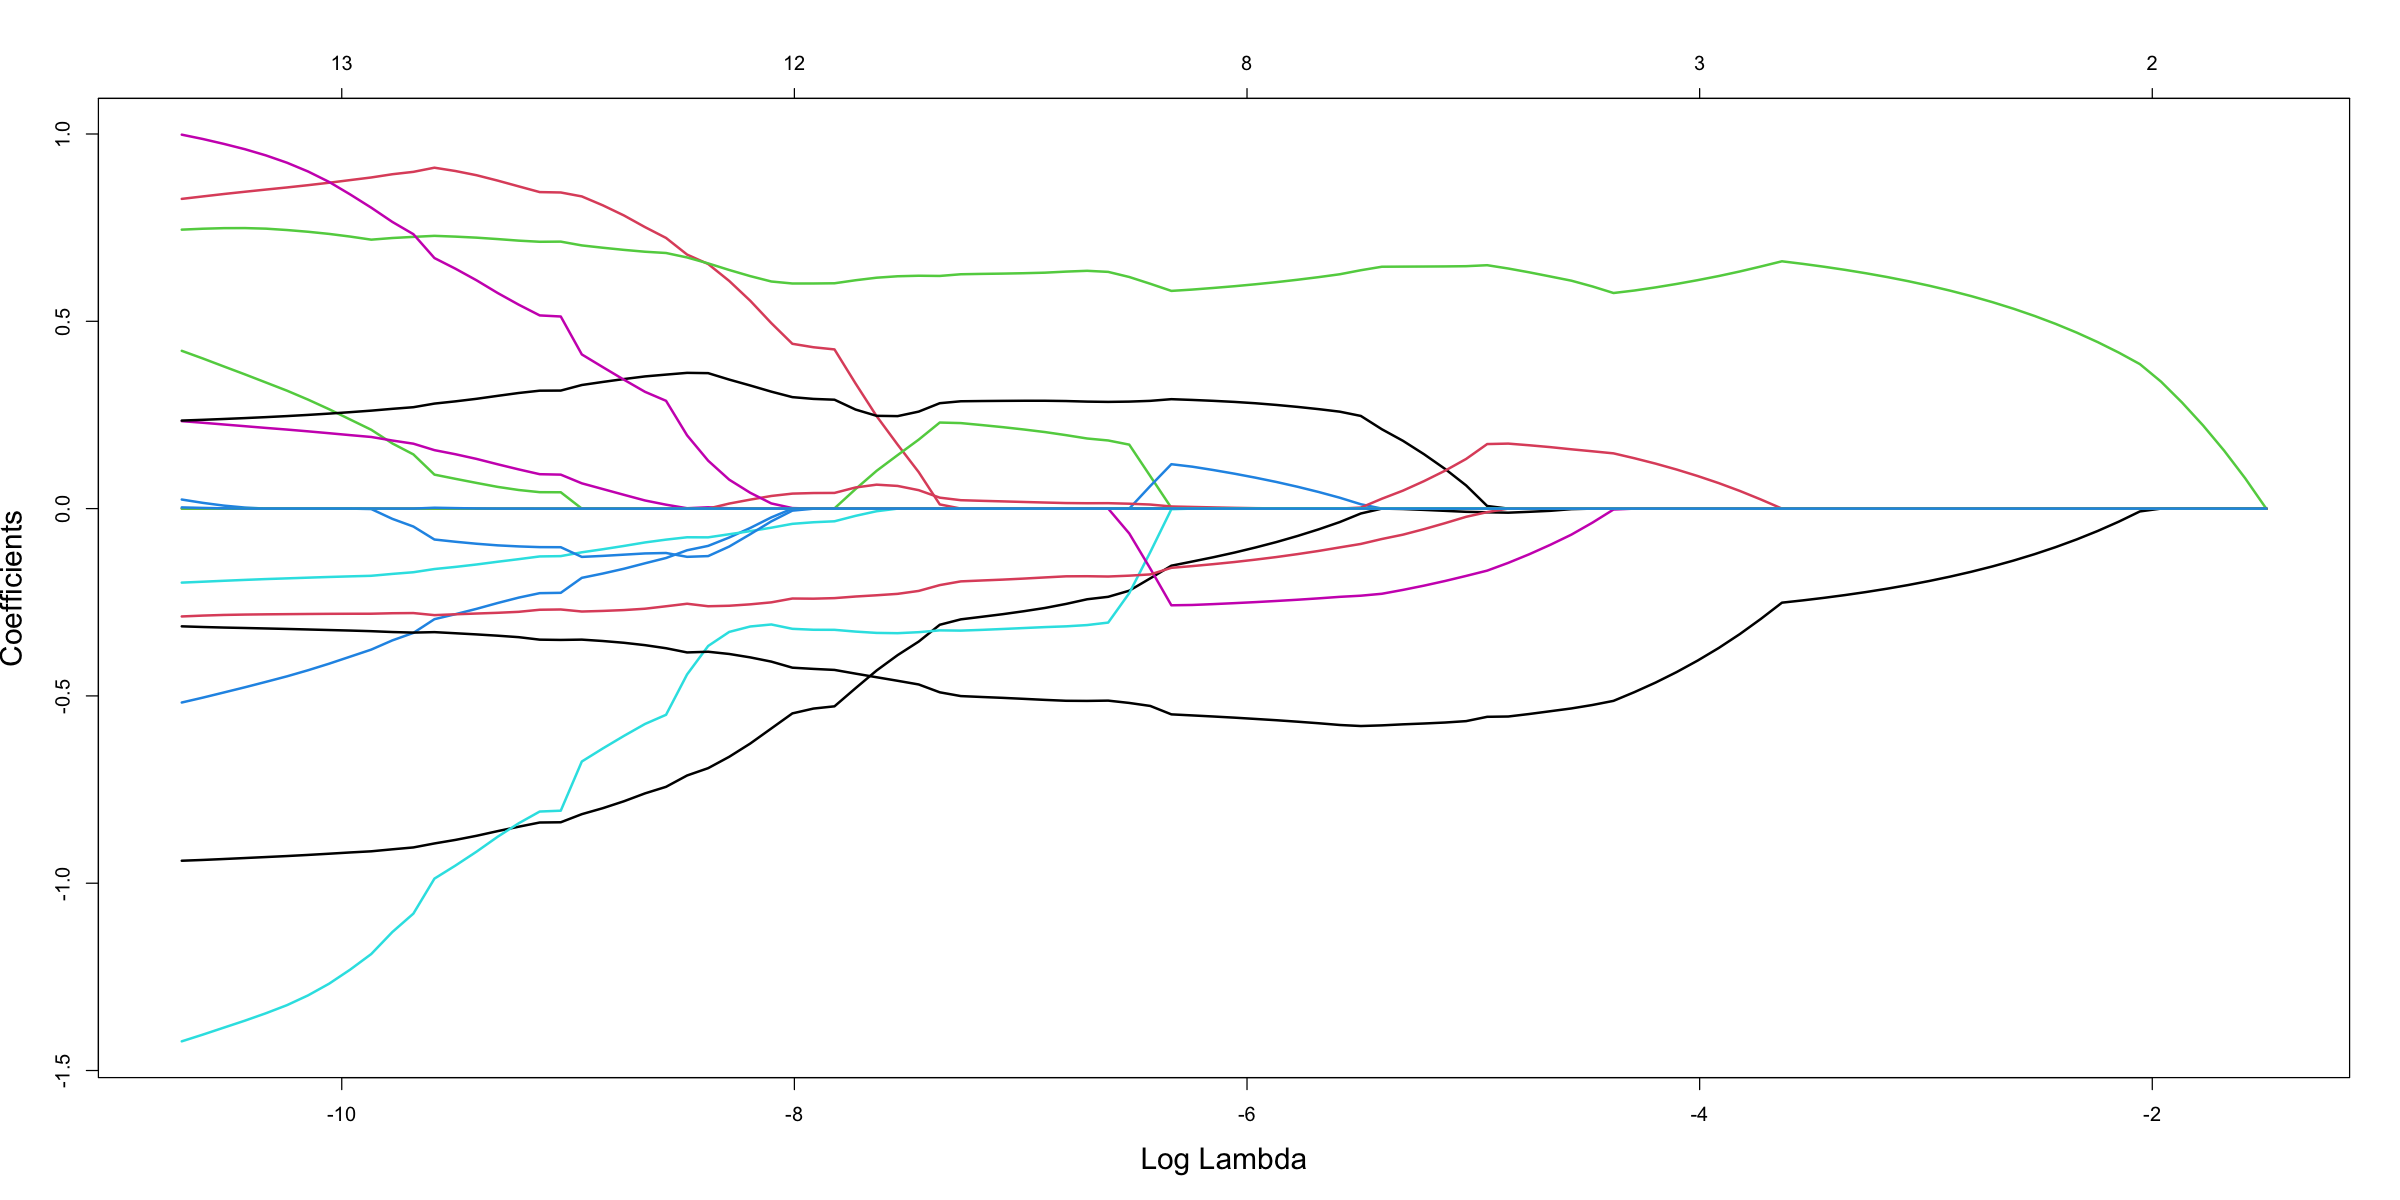
\includegraphics[width=7cm]{Figure/4.2.3-PPR-ridge-trance.png}
  \end{subfigure}
  \begin{subfigure}{7.5cm}
    \centering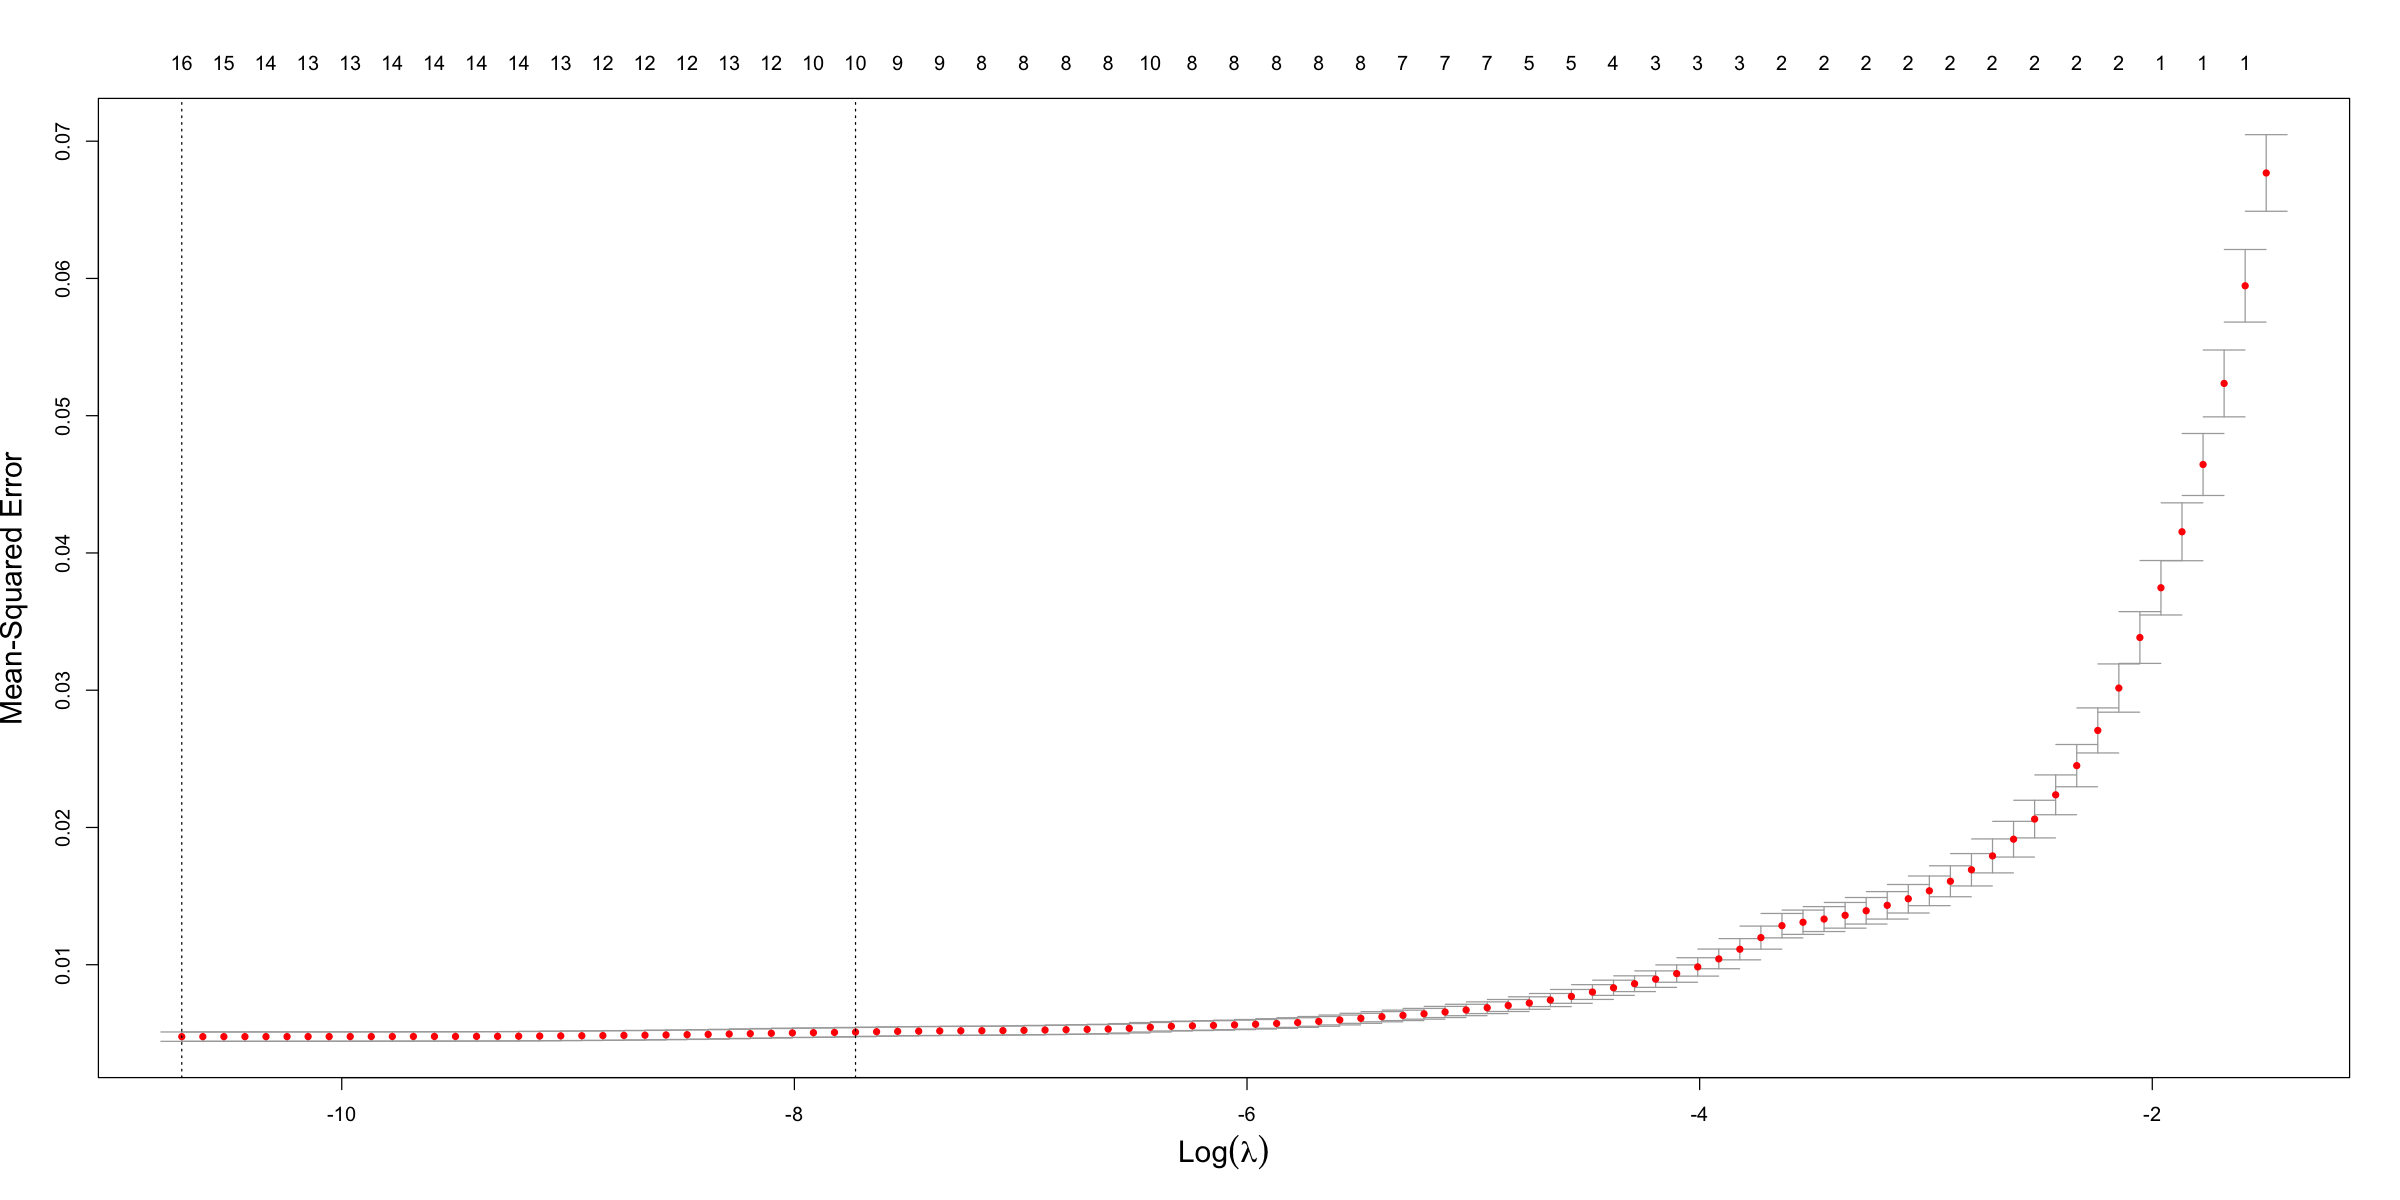
\includegraphics[width=7cm]{Figure/4.2.3-PPR-Log-Lambda-vs-Testing-Error.png}
  \end{subfigure}
  \caption{Left: Ridge trace diagram of Penalised Polynomial Regression. Right: Log Lambda vs Testing Error diagram of Penalised Polynomial Regression.}
  \label{4.2.3-NEW-PPR-ridge-trance-Log-Lambda}
\end{figure}

According to the following results in Table \ref{4.2.2-PPR-para}, no features are removed in this model with min, and its MSE is 0.00448. In 1se, 6 features are removed and its MSE is 0.00483. At the cost of small precision loss, the model can be greatly simplified, which is exactly the purpose of the 1se option of Lambda.

\begin{table}[htbp]
  \centering
  \footnotesize
  \begin{tabular}{p{2cm} | c | c}
  \toprule
  Coefficients: & min & 1se\\ %row 1
  \hline
    & 1 & 1\\
  (Intercept)& 7.817628e-01 & 0.7495621617\\
  Rainfall   & -9.399989e-01 & -0.5338097486\\
  Rainfall.2 &  8.267722e-01 & 0.4307466064\\
  Rainfall.3 &  4.211873e-01 & .\\
  Rainfall.4 & -5.176367e-01 & .\\
  Daylight   & -1.975953e-01 & -0.0364294056\\
  Daylight.2 &  2.334835e-01 & .\\
  Daylight.3 &  2.349987e-01 & 0.2928271727\\
  Daylight.4 &  1.117847e-05 & 0.0415480304\\
  Ozone      &  7.446573e-01 & 0.6009477148\\
  Ozone.2    &  2.420938e-02 & -0.0002389955\\
  Ozone.3    & -1.422105e+00 & -0.3234189416\\
  Ozone.4    &  9.982037e-01 & .\\
  MinTemp    & -3.142767e-01 & -0.4278954907\\
  MinTemp.2  & -2.878996e-01 & -0.2404459826\\
  MinTemp.3  &  1.936775e-05 & .\\
  MinTemp.4  &  3.213799e-03 & .\\
  \bottomrule
  \end{tabular}
  \caption{Hyper-parameters of Penalised Polynomial Regression.}
  \label{4.2.2-PPR-para}
\end{table}



By comparing the fitting diagram (Figure \ref{4.2.3-PPR-min-1se}) of two results, it was found that the results were similar, which further proved that the influence of 1SE value on the accuracy of the model was almost negligible. At the same time, compared with Linear Regression, the fitting results were significantly better as polynomial regression brought more flexibility to the model.

\begin{figure}[htbp]
\center
  \begin{subfigure}{7.5cm}
    \centering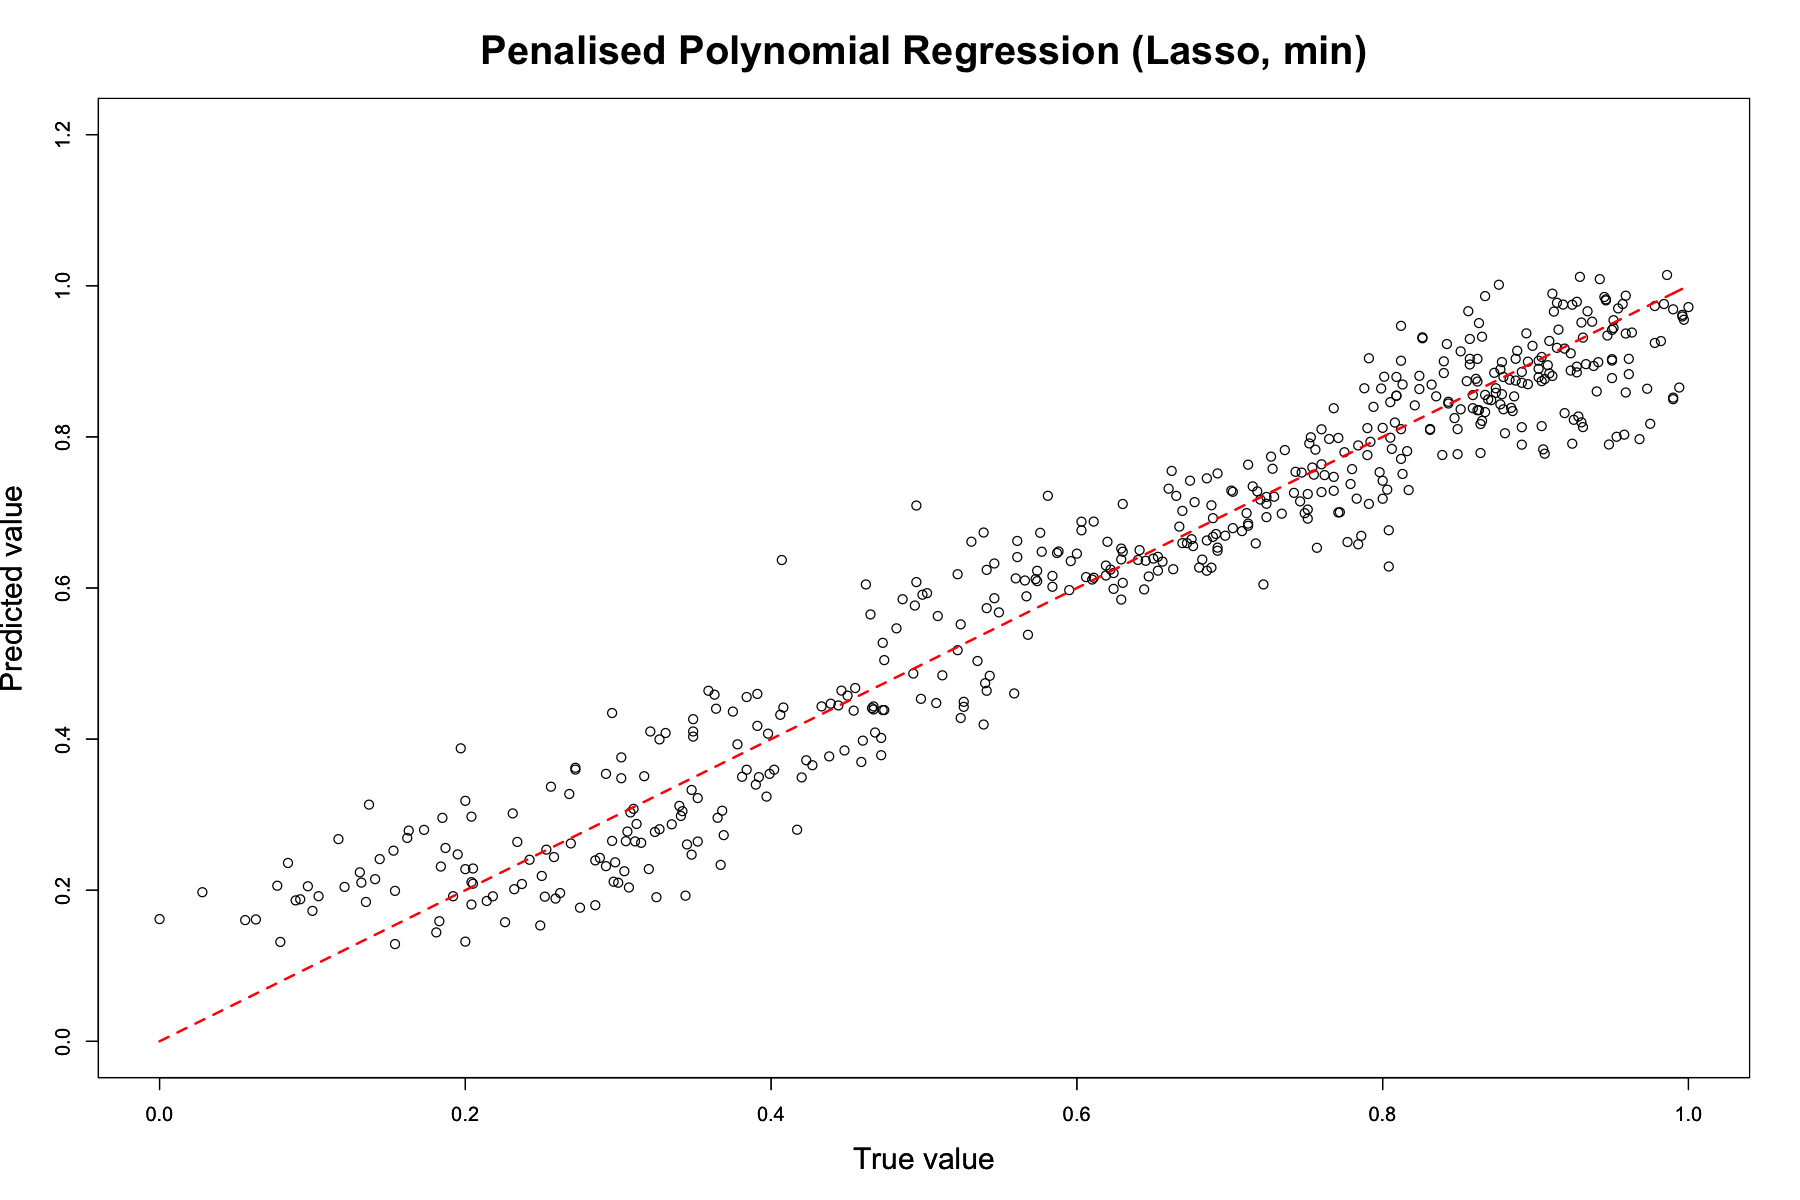
\includegraphics[width=7cm]{Figure/4.2.3-PPR-min.png}
  \end{subfigure}
  \begin{subfigure}{7.5cm}
    \centering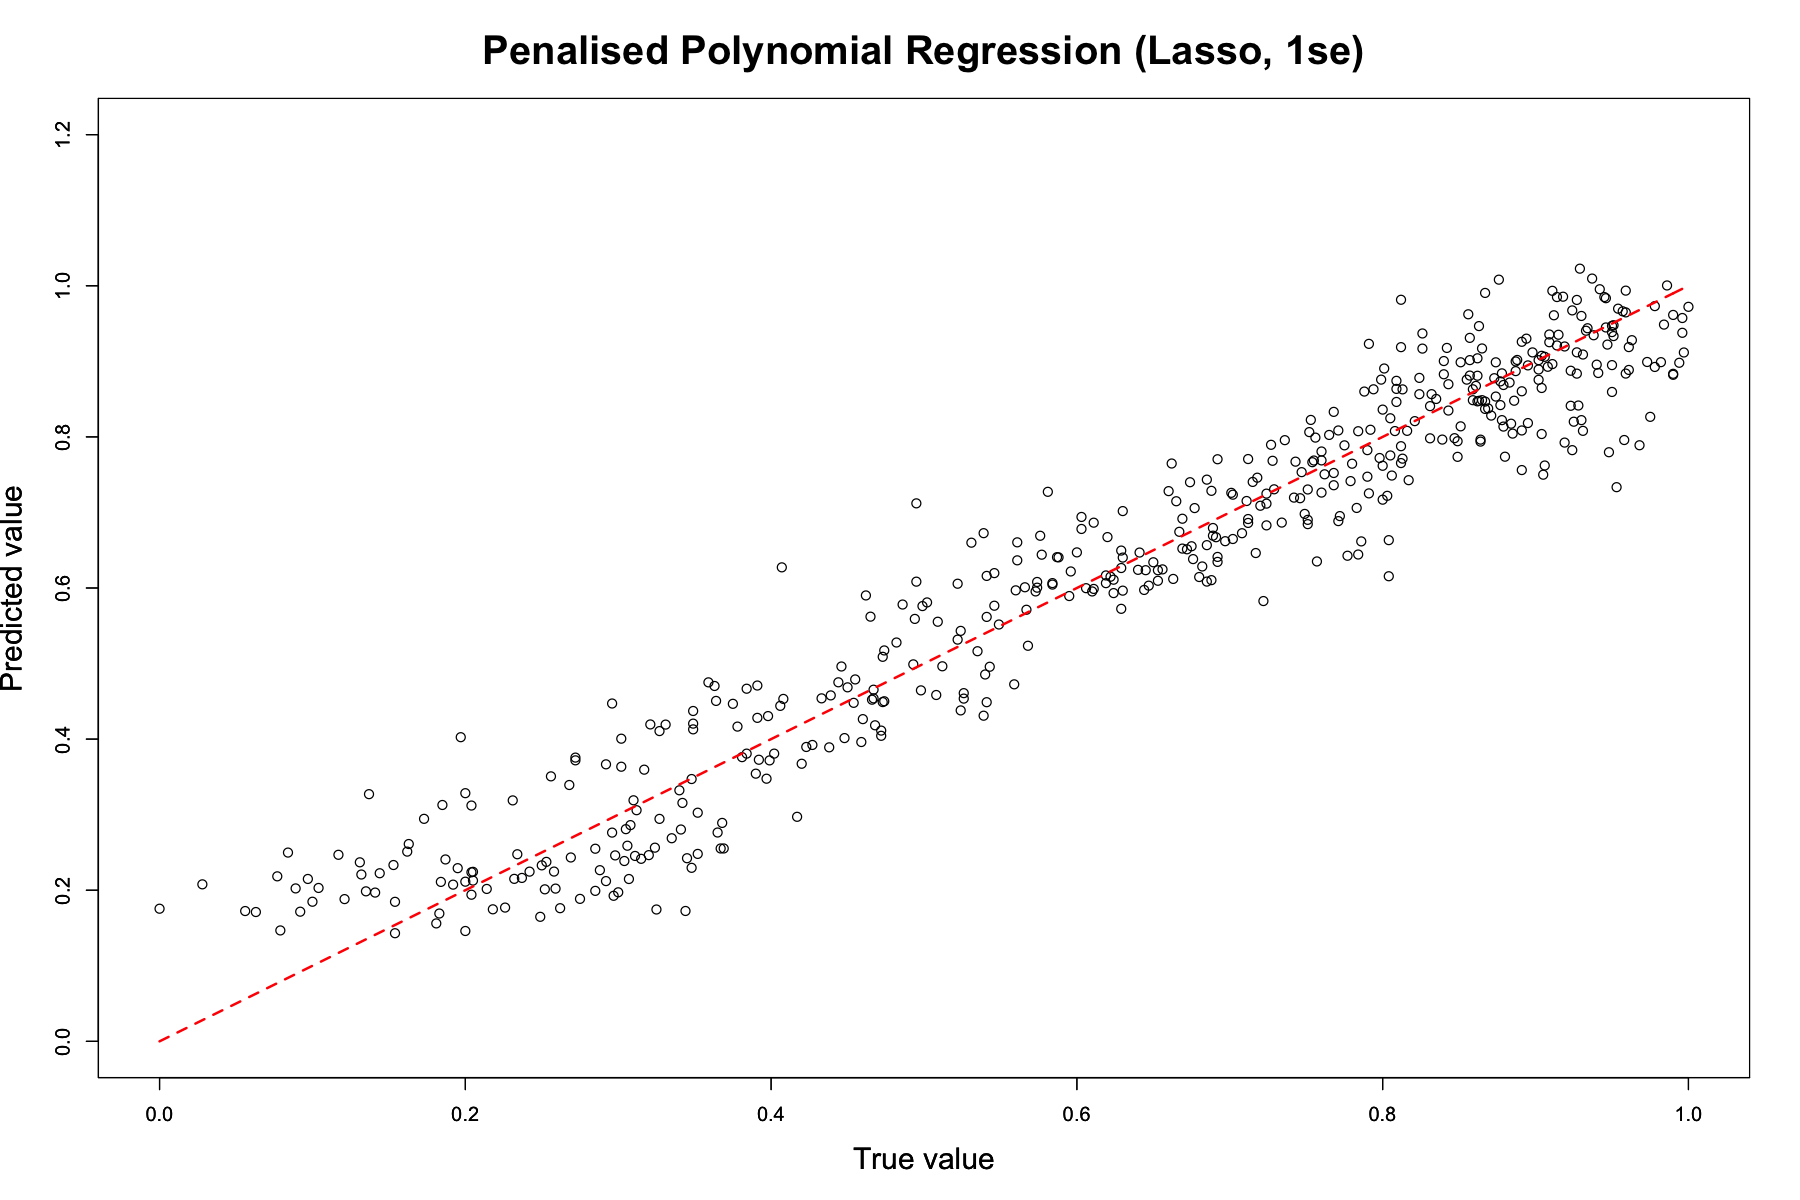
\includegraphics[width=7cm]{Figure/4.2.3-PPR-1se.png}
  \end{subfigure}
  \caption{\textbf{Left}: The predicted Arctic sea ice extent value vs the real Arctic sea ice extent value with \textbf{Penalised Polynomial Regression} (Lasso, \textbf{min}). The red referenced dotted line represents the straight line y=x. Mean Square Error (MSE) is \textbf{0.00448}. \textbf{Right}: The predicted Arctic sea ice extent value vs the real Arctic sea ice extent value with \textbf{Penalised Polynomial Regression} (Lasso, \textbf{1se}). The red referenced dotted line represents the straight line y=x. Mean Square Error (MSE) is \textbf{0.00484}.}
  \label{4.2.3-PPR-min-1se}
\end{figure}

\newpage